% WARNING README TO COMPILE
% YOU *MUST* USE PDFLATEX, NOT JUST LATEX, OR ELSE IMAGES WILL NOT APPEAR
\documentclass[a0]{a0poster}
\usepackage{tabularx}
\usepackage{palatino}
\usepackage{epsfig}
\usepackage{alltt}
\usepackage{graphicx,epsfig}
\usepackage{amsmath,color,amsthm,dsfont,amssymb,multirow}
\newcommand{\mybf}[1]{\mathbf{#1}}

\def\vlambdao{{\boldsymbol{\lambda}_1^T}}
\def\vlambdat{{\boldsymbol{\lambda}_2^T}} 
\def\vfo{\boldsymbol{f}_1}
\def\vft{\boldsymbol{f}_2}

\definecolor{DarkBlue}{rgb}{0.1,0.1,0.5}
\definecolor{Black}{rgb}{0.0,0.0,0.0}
\definecolor{Red}{rgb}{0.9,0.0,0.1}
\definecolor{DarkBlue2}{rgb}{0.00,0.08,0.6}
\definecolor{DarkRed2}{rgb}{0.6,0.00,0.08}
\definecolor{DarkGreen2}{rgb}{0.00,0.6,0.08}
%\newcommand{\yang}[1]{{\color{DarkBlue}\par{\Large\bf #1}\par}}
\newcommand{\yang}[1]{{\color{DarkBlue}\par{\bf #1}\par}}
\newcommand{\myBlue}[1]{{\color{DarkBlue}#1}}
\newcommand{\myGreen}[1]{{\color{DarkGreen2}#1}}

% For debugging, force all o/p to be on one page, even though it will overrun.
% Remove this to print final copy
% \textheight200in

\parindent=0pt
\newcommand{\rect}[2]{
\mbox{\begin{minipage}{#1}
\framebox[#1]{\rule{0pt}{#2}}
\vspace{-#2}
\vspace{-\baselineskip}
\vspace{-10pt}
\end{minipage}
}}

\def\m#1{{\tt #1}}
\def\v#1{{\bf #1}}
\newcommand{\colvec}[1]{\left( \begin{array}{c} #1 \end{array} \right)}
\newcommand{\awfwbox}[1]{\parbox{\textwidth}{\hspace*{\fill}#1\hspace*{\fill}}}
\newcommand{\epswide}[2]{\psfig{figure=#2,width=#1\textwidth}}
\newcommand{\epshigh}[2]{\psfig{figure=#2,height=#1\textwidth}}
\newcommand{\T}{{\cal T}}
\newtheorem{thm}{Theorem}

%\renewcommand{\paragraph}[1]{\vspace{1cm}\par{\Large\bf #1}\par}
\renewcommand{\paragraph}[1]{{\color{DarkRed2}\vspace{1cm}\par{\LARGE\bf #1}\par}}

\newcommand{\awfhline}{\rule{\textwidth}{1pt}}

\newlength{\colwidth}
%\setlength{\colwidth}{0.181\textwidth}
\setlength{\colwidth}{0.31\textwidth}

\newcommand{\col}[1]{
\fbox{
\begin{minipage}[t]{\colwidth}\raggedright\large
#1
\end{minipage}
}
}

\newcounter{elist}
\newenvironment{awfitemize}[1]{\begin{list}{#1}{
 \usecounter{elist}
 \setlength{\leftmargin}{2mm}
 \setlength{\labelwidth}{4mm}
 \setlength{\labelsep}{.1mm}
 \setlength{\itemindent}{0pt}
 \setlength{\rightmargin}{0pt}
}}{\end{list}}
% 
% \renewenvironment{itemize}{\awfitemize{$\bullet$\hfill}\setlength{\labelwidth}{2mm}}{\endawfitemize}
% \renewenvironment{enumerate}{\awfitemize{\arabic{elist}.}}{\endawfitemize}
% 

%%%%%%%%%%%%%%%%%%%%%%%%%%%%%%%%%%%%%%%%%%%%%%%%%%%%%%%%%%%%%%%%%%%%%%%%%%%%%
\newcommand{\awfp}[2]{{
\tiny\begin{tabular}{c}
\epsfysize=30mm\epsfbox{#1}\\
\hfill#2
\end{tabular}
\hspace{-1em}
}}

\begin{document}
\small
\thispagestyle{empty}
\rect{\textwidth}{\textheight}

\begin{tabularx}{\textwidth}{cXc}
\begin{minipage}{4in} \end{minipage}&
\centering \begin{minipage}{25in}
\begin{center}
\vspace{0.5cm}
{\color{DarkRed2}{\Huge\bf An Evaluation of the Statement Deletion Mutation Operator in Real-World Python Projects}}\\
\vspace{0.8cm}
{\color{DarkBlue}{\LARGE Shan Cao, Dongyuan Liu}}\\
\end{center}
\end{minipage} &
\begin{minipage}{4in} \end{minipage}
\end{tabularx}

\begin{center}\col{
\paragraph{Introduction}
	{\LARGE
		Many open-source libraries use test coverage as a measurement of test suite quality. However, test coverage only guarantee the code is being executed when running the tests, it does not check that the tests are able to detect real faults.
		To get deeper knowledge of the flaws, running test set against slightly modified versions of programs is one approach. This technique is called \emph{mutation testing}.

		In this paper, we specifically evaluate the statement deletion mutation operator (SDL). We evaluate on real-world Python projects and their test suites.
	}

\awfhline

\paragraph{MutPy}
	{\LARGE
	\emph{MutPy} is a mutation testing tool for Python projects. We use it to compute and compare the result of SDL and experimental mutation. This tool has not received any updates since 2014. To make it compatible to recent libraries, we updated it to support Python 3.5 and fixed some issues in loading unit tests before starting the experiment. The version we are using is in this forked repository.
	}
	\vspace{0.5cm}

\awfhline

\paragraph{Python projects for evaluation}
	\vspace{0.5cm}
	\begin{tabular}{|l|r|l|}
	\hline
	{\bf Project} & {\bf LOC} & {\bf Description} \\
	\hline
	python-magic      & 391   & A Python wrapper for libmagic \\
	Delorean          & 1991  & A library for datetimes in Python \\
	FuzzyWuzzy        & 1352  & Fuzzy string matching in Python \\
	pangu.py          & 446   & Paranoid text spacing in Python \\
	shortuuid         & 355   & A generator library for UUIDs \\
	python-slugify    & 425   & Returns unicode slugs \\
	python-nameparser & 4027  & Parse human names into components \\
	python-markdown   & 8199  & A Python implementation of Markdown \\
	sqlparse          & 19434 & A non-validating SQL parser for Python \\
	\hline
	\end{tabular}

}
\col{
	\vspace{0.5cm}
	{\LARGE
	\begin{center}
		Mutation Operators Supported by MutPy
		\begin{tabular}{c | c}
			Operation & Description \\ \hline
			\texttt{AOD} & arithmetic operator deletion \\
			\texttt{AOR} & arithmetic operator replacement \\
			\texttt{ASR} & assignment operator replacement \\
			\texttt{BCR} & break continue replacement \\
			\texttt{COD} & conditional operator deletion \\
			\texttt{COI} & conditional operator insertion \\
			\texttt{CRP} & constant replacement \\
			\texttt{DDL} & decorator deletion \\
			\texttt{EHD} & exception handler deletion \\
			\texttt{EXS} & exception swallowing \\
			\texttt{IHD} & hiding variable deletion \\
			\texttt{IOD} & overriding method deletion \\
			\texttt{IOP} & overridden method calling position change \\
			\texttt{LCR} & logical connector replacement \\
			\texttt{LOD} & logical operator deletion \\
			\texttt{LOR} & logical operator replacement \\
			\texttt{ROR} & relational operator replacement \\
			\texttt{SCD} & super calling deletion \\
			\texttt{SCI} & super calling insert \\
			\texttt{SIR} & slice index remove \\
		\end{tabular}
	\end{center}
	\vspace{0.5cm}

	\awfhline

	\begin{center}
		Experimental Mutation Operators
		\begin{tabular}{c | c}
			Operation & Description \\ \hline
			\texttt{CDI} & classmethod decorator insertion \\
			\texttt{OIL} & one iteration loop \\
			\texttt{RIL} & reverse iteration loop \\
			\texttt{SDI} & staticmethod decorator insertion \\
			\texttt{SDL} & statement deletion \\
			\texttt{SVD} & self variable deletion \\
			\texttt{ZIL} & zero iteration loop \\
		\end{tabular}
	\end{center}
	}
}
\col{
	\vspace{0.5cm}
	\begin{center}
		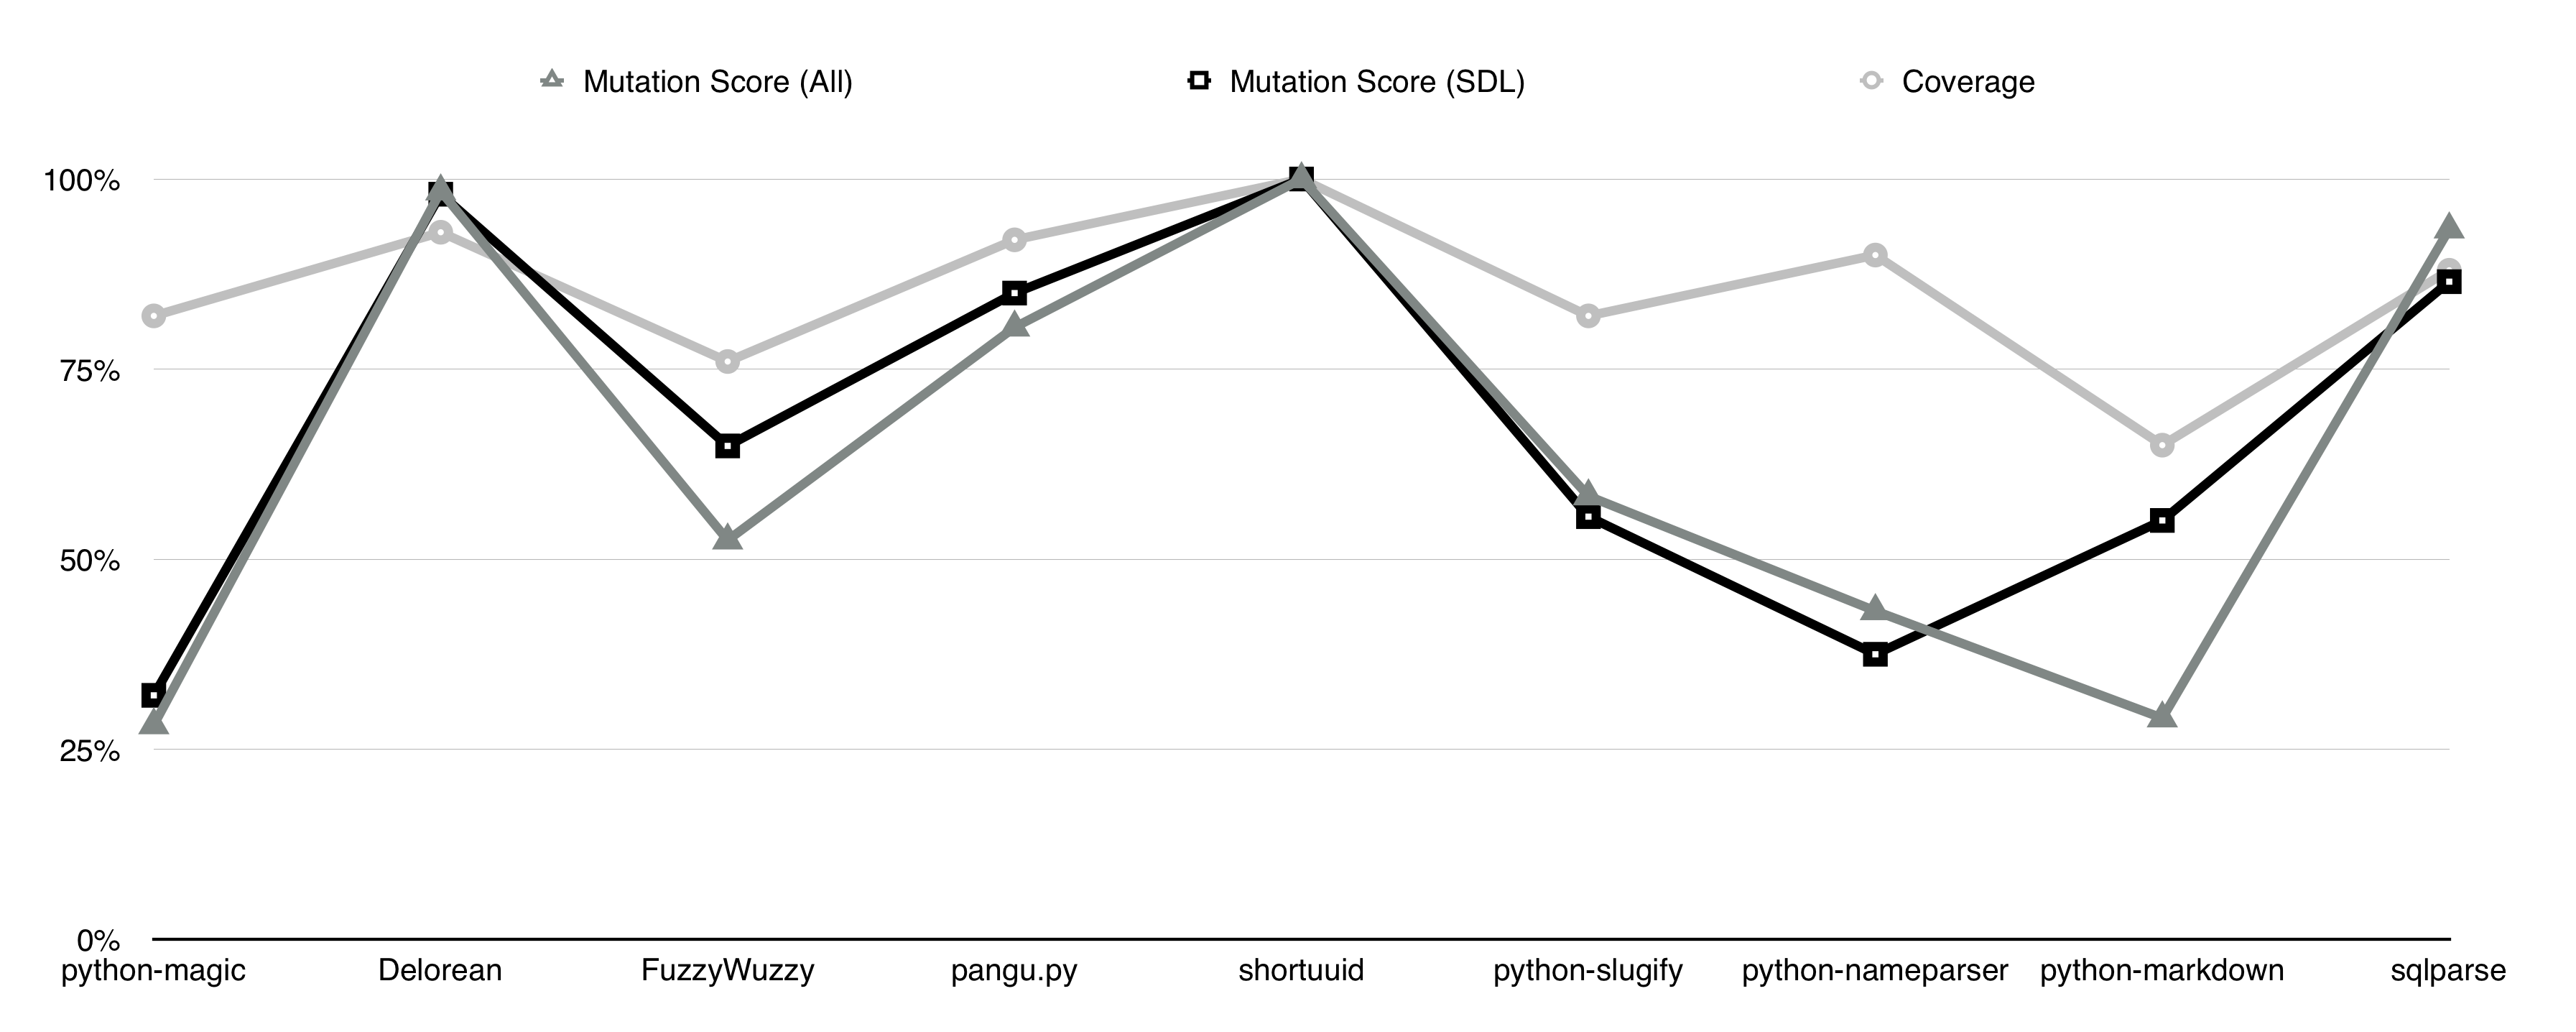
\includegraphics[width=34cm]{figures/score.png}	
	\end{center}
	\begin{center}
		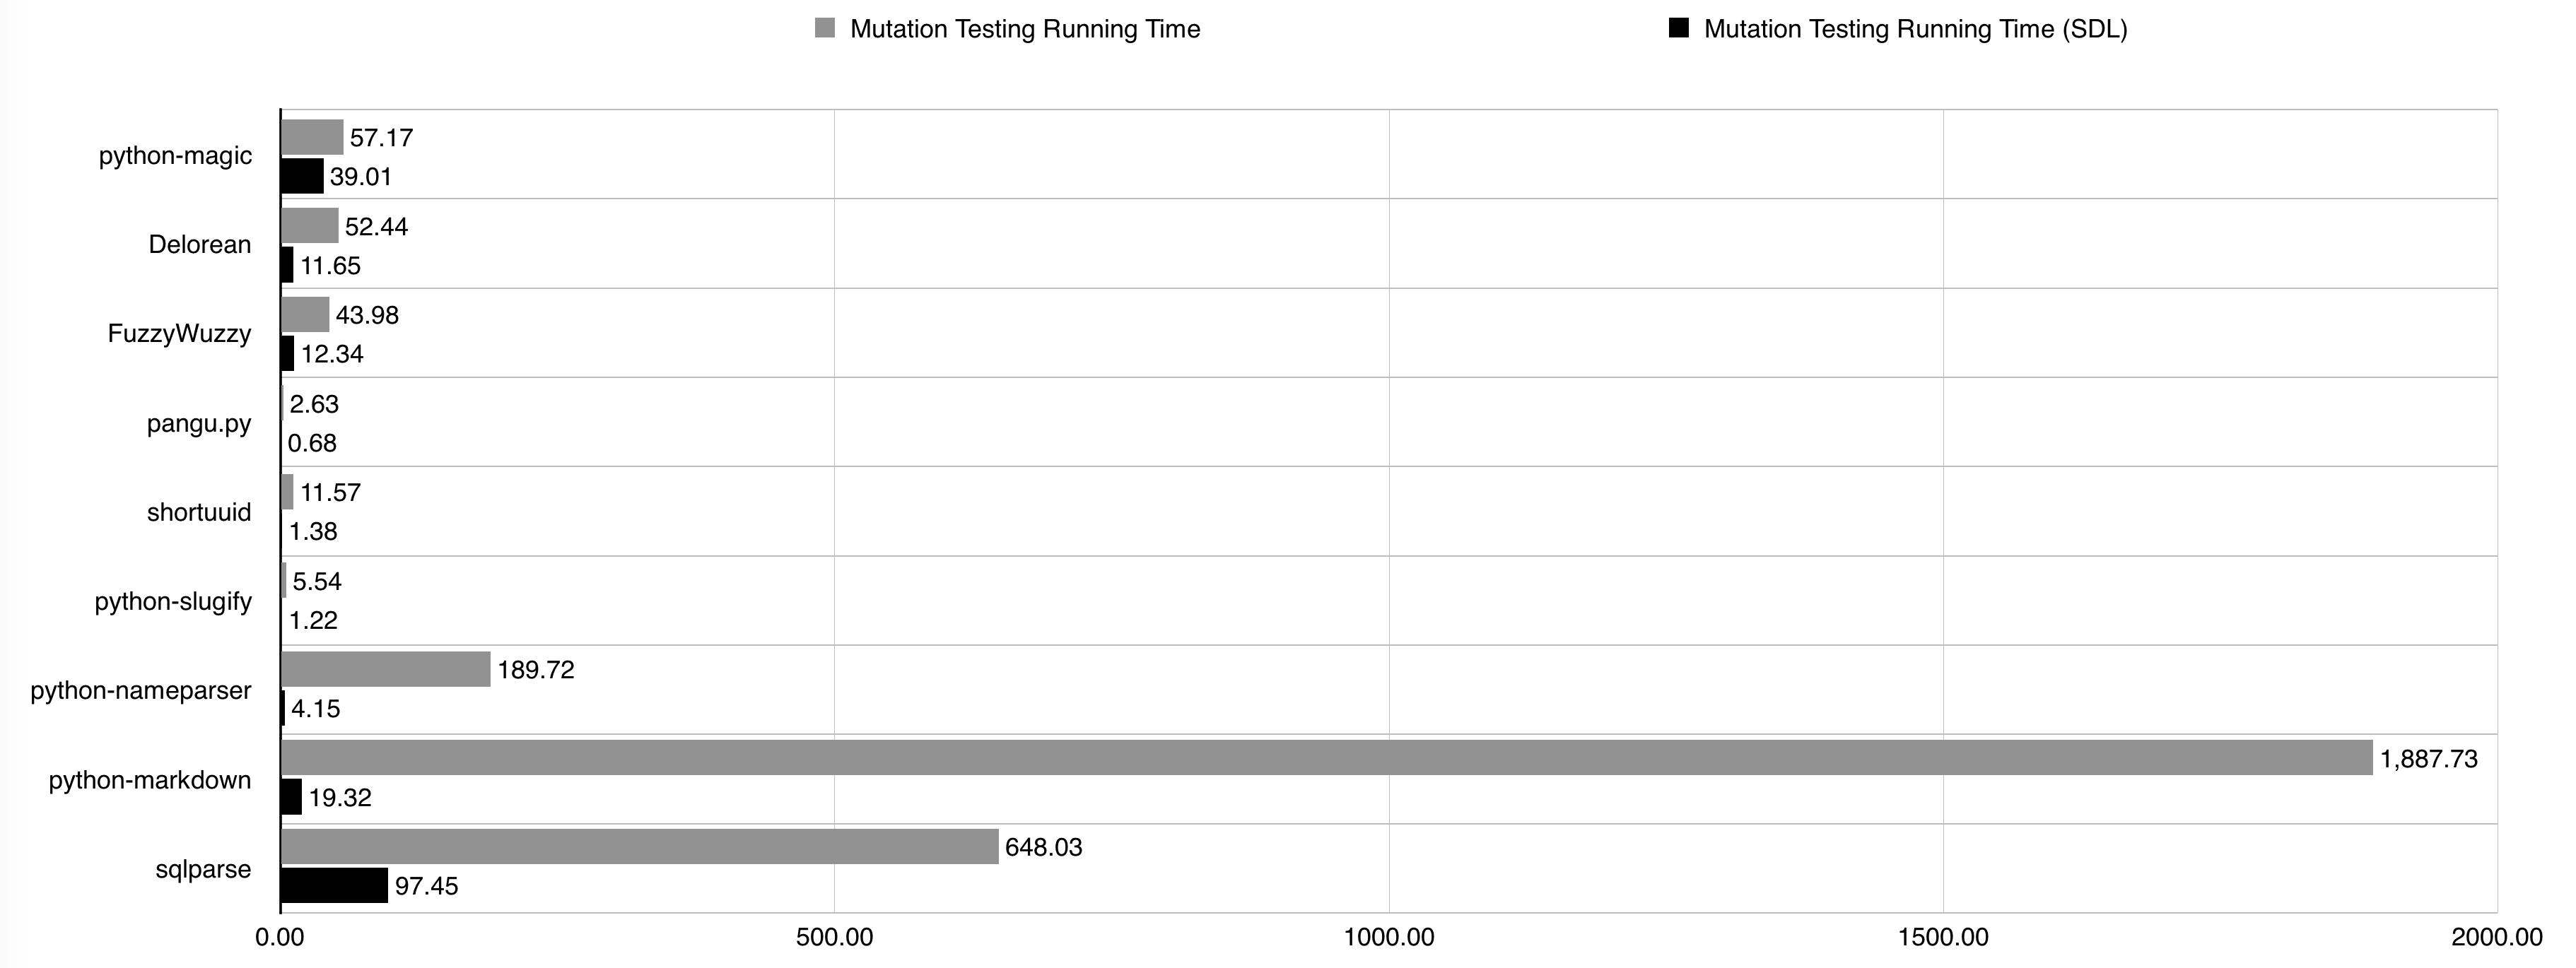
\includegraphics[width=34cm]{figures/time.png}
	\end{center}
	SDL-mutation compared to full mutation
	\awfhline
	\paragraph{Further Work}
		{\LARGE
			\begin{itemize}
				\item Currently MutPy only loads unit tests based on the Python standard unittest module. However, there are many popular Python projects that do not use the unittest module.
				\item  A big issue for mutation testing with SDL operator is that after removing a statement, it could form an infinite loop. We can record the running time for all the tests before running mutation testing. For each test, we set the timeout separately based on its running time.
				\item Mutation testing is slow because it runs the whole test suite for every mutant. We can run a subset of tests that covers the mutant.
				\item Investigate the relevancy between survived mutants and bugs.
				\item Explore appropriate use cases for mutation testing.
			\end{itemize}
	}
}
%
\end{center}

\vfill
\begin{center}
{\color{DarkBlue}\LARGE \hspace{5cm}CMPT 479 Term Project, 2016 Spring\hspace{5cm}}\\
\end{center}

\end{document}
